\chapter{Introduction and Background}\footnotetext{some content in section 1.1 and  section 1.2 of  this  chapter is adapted from Dou, Yong, Kiran Dhatt-Gauthier, and Kyle JM Bishop. "Thermodynamic costs of dynamic function in active soft matter." Current Opinion in Solid State and Materials Science 23.1 (2019): 28-40.See appendix for the full text of this paper}
Robotics is in the spotlight of coming industry 4.0 era \cite{lasi2014industry}.Highly automatic robots will largely increase the productivity and efficiency in many areas such as manufacturing, transportation and retailing. 
It is predicted that 47$\%$ percent of jobs will be replaced by robotics in two decades. \cite{frey2013future}
Research on robotics almost include all part of science and engineering fields from the data science, machine learning to the material science and biology. Lots of current design and development of robotics are inspired from nature to achieve the animal/human-like functions, for example  the famous  bio-inspired robot SPOT\textregistered  by Boston Dynamics \cite{yang2019ten} can perform like dogs  to climbs stairs and run on rough terrain with very impressive ease. Normal robots are usually in the size of meters. However, this dissertation is going to focus on robots with a much smaller size around microns(1$\mu m=10^{-6} m$) called \textbf{colloid robots}. Colloid robots are at the same size of microorganism and living cells,and are designed to mimic similar living functions in a colloidal scale.  

In the first chapter, some basic knowledge of colloid robots are introduced as well as the state of arts research on colloid robots. We gave the  classification for colloid robots based on different automation level(from level 0 to level 6). Chapter 2 showed  an example example developed by us to a achieve level 1 automation with electrostatic actuation. Contact charge electrophoresis(CCEP) uses the repeating electrostatic charging and actuation to drive   
continuous autonomous motion of anisotropic colloids particles with very high speed and low power input. In Chapter 3, we  design an experiment system that conductive  colloids particles can interact with each other to generate dynamic travelling waves. A modified Kuramoto model treating colloids as phase oscillators is proposed to explain the experiment observation. Chapter 3 provide a pathway to realize level 2 automation for colloid robots. In Chapter 4, a theoretical toy model is introduced to design level 4 automation colloid robots. The colloid robots are interact with the environment and make decisions based on local information by changing their shapes to reach the global navigation behaviors. This toy model provides an design and optimization frames for autonomous navigation in colloid robots. Chapter 5  shows a system in which  magnetic actuated colloid robots can  finish level 4 autonomous navigation. We develop physical mode of     magnetic actuated colloid robots and optimize the design space to navigate the motion of magnetic rollers.  Preliminary experimental results are also discussed in chapter 5. In Chapter 6, future research directions  are proposed  to guide  ultimate realization of  automation level 5 and 6 colloidal robots. 

\section{Bio-inspired Colloids Robots}
Living cells or microorganism(e.g. bacteria) are the smallest unit of life. Although these smallest units is only in the size of colloid particles(most cells' size are in the range from 1$\mu m$ to 100$\mu m$), living cells can perform all the basic remarkable dynamics functions of life. For example, plan cells capture energy from sunlight and convert it into chemical fuels and structural materials; muscle cells powers organisms to move and to transport matter throughout their interiors; the cytoskeleton incessantly reconfigures its structural components, enabling cells to adapt their mechanical properties to their environment; neural cells uses complex signaling networks to sense environmental inputs and compute intelligent outputs. Perhaps most remarkably, all cells can grow and replicate to escape the unrelenting pull toward thermodynamic equilibrium (i.e., death).  All of these functions ---and the many others not listed---would be highly desirable to achieve in an small artificial robotics system, or called as colloids robots. \textbf{Colloids robots refers to the colloid size units which can perform life-like autonomous behaviors including motion, navigation, sensing, communication or even high level cognition}.  Colloids robots are bio-inspired and trying to mimic living cells, however colloids robots can also designed to have better performance and more complex functions than real living cells. A qualified colloids robots is designed to finish colloid scale tasks with high accuracy and precision at a reasonable energy efficiency.
\section{Why colloids Robots are different and could be hard to realize}
Although colloids robots still follow the basic control feedback of normal size robots: sensing, computation and actuation, these components of the control loop are hard to realize with respect to the size limitation and totally different physics in small scale. 

\textbf{Size limitation}. In addition to the three basic components( sensor,actuator and processor) in the feedback loop, a robot also need power supplies, manipulators with joints and a body frame etc. Even for a simple clean robots, there are around 100 parts inside. It is not possible to integrate all of these complex components in a micron size(a micron size particle on a cleaning robot is just like a human standing on the earth) particle if we follow the common way to build a normal size robot. 

\textbf{Physics limitation}. Physics in a small scale and squishy  environment is very different from our normal size world, where everything becomes noisy and sticky. First, in the colloidal scale, Brownian motions largely affect the dynamics of colloidal particles, adding stochastic influence to the robotics. These thermal motions increase the difficulties in controlling colloid robot's accuracy and precision. Second the inertia totally disappear in the small scale as the Reynolds number of the colloid robot's system approach 0.  Reynolds number presents the ration of inertia and viscosity represented as
\begin{equation}
    Re=\frac{\rho v l}{\mu}
\end{equation}
where $\rho $ is the density of fluid environment, v is the velocity of particle, l is the size of particle. $\mu$ is the  viscosity of fluid. In the colloid scale, both size and speed of particle are much smaller than 1 leading to the Reynolds number approach 0. The absence of inertia means all of the actuation method in normal size robots based on inertia will no longer work. This interesting  motion restriction in low Reynolds number is called Scallop
theory and was first discussed by Edward Purcel(Professor Prucel was famous for his independent discovery of something else(nuclear magnetic resonance,NMR), which brought him a Nobel prize) \cite{purcell1977life}. As shown in \textcolor{red}{fig XXX},  Scallop Theorem states that a swimmer that exhibits time-symmetric motion cannot achieve net displacement in a low Reynolds number fluid environment because all the motion is time reversal like the open and close of a scallop. New actuation methods must be applied to drive motions for colloid robots.

To solve the above mentioned problems and design colloid robots, researchers got inspired from living. The dynamic functions of living cells require integration of structures and processes to drive material organization in space and time. For example in muscle cell,  the coupling of complex structures(kinesin motor protein) and dissipative processes (ATP hydrolysis) can generates mechanical work. \textcolor{red}{see fig XXX}

Thanks to the development of nano/micro scale fabrication in semiconductor industry, we can now create materials with heterogeneous structure and composition on length scales spanning molecular to macroscopic dimensions with chemical synthesis, lithography, deposition and etching. These technologies can be directly transplanted to the fabrication process of colloidal robots. In addition to structural and material complexity, the artificial dissipation process(or actuation process) for colloid robots  can be generated  with chemical reaction, external field(electric, magnetic, acoustic or fluid flow) to generate motion by by break the time reversal physics. For past decade, lots of research has been conducted to design colloidal robots or study the fundamentals of colloid robots. Colloid robots is now a very hot emerging interdisciplinary field attracting many scientist from math, physics, chemistry, biology and engineering. The states of art of  research approach to colloid is reviewed on\textcolor{red}{section , section }
\section{The importance of  sensing in colloid robots}
modular, self awareness, make difference between force and 

reprogrammable 
 programmed motions
  AI we call such things reflex agents. 
  
  \textbf{repurposable}
  
  Industrial robot as defined by ISO 8373:

An automatically controlled, reprogrammable, multipurpose manipulator programmable in three or more axes, which may be either fixed in place or mobile for use in industrial automation applications.

Reprogrammable: whose programmed motions or auxiliary functions may be changed without physical alterations;

Multipurpose: capable of being adapted to a different application with physical alterations;

Physical alterations: alteration of the mechanical structure or control system except for changes of programming cassettes, ROMs, etc.

Axis: direction used to specify the robot motion in a linear or rotary mode

For example, let's think about a welding operation that takes place in a car factory. This operation could be done with a custom machine that lowers welding elements into place at the appropriate place on the car. Or we could install a robot arm, put a welder on the end of the arm, and teach (program) it where to weld. When a new model of car comes along, we can teach it the new weld points. If we no longer need the welding operation, we can move the robot somewhere else, put a new tool on the end of the arm, and teach it to paint or to screw in a bolt.

 If you can't easily re-purpose your machine to do something completely different by reprogramming (and perh
 
 Animal -> Robot
Plant -> Machine

\section{Automation level of Colloid Robots}
Before the review of current approach to the colloid robots, 
we give the  automation level definitions for colloids robots,  analogy to the Levels of driving automation\cite{taeihagh2019governing}. This level definition is proposed to guide the research road-map for colloid robots.
\begin{itemize}
    \item Level 0 No Automaton: This level of automation means colloid robots cannot do anything autonomous. All the conventional colloid particles (even with complex structures and components) belong to this level. These particles are in the equilibrium state.
    \item Level 1 Autonomous  Motion: At level 1, individual colloid robot can continuous harness the energy from the environment to power autonomous motion. This is the entry autonomous level for colloid robots. Although colloid robots at level 1 can move, they can't move with any complex tasks such as navigation and communication.
    \item Level 2 Autonomous Coordination: Group of colloid robots can interact with each other to perform swarm behaviors and generate patterns. Colloid robots begin to show the sensing function at Level 2 via interacting with each other. But this kind is sensing is passive  and still lack the ability to make initiative decision/reaction based on sensing. 
    \item Level 3$^{-}$ Supervised Autonomous Navigation (Eyes on): colloid robots' motion can be guided with the outside computer vision feedback system. At Level 3$^{minus}$, the sensor are outside the colloid robot as the observation microscope, camera. The decision makers and respond mechanism are supervised by outside computer vision algorithm. Colloid robots cannot finish navigation task independently in a small scale.
    \item Level 3$^{+}$ Unsupervised Autonomous Navigation (Eyes off): Colloid robots can finish the sensing-computation-actuation feedback loop independently without the outside devices to supervise. Autonomous navigation in Level 3 $^{+}$ satisfied the basic autonomous requirement for a normal robot. Autonomous level higher than level 3 will enter the area of artificial intelligent.
    \item Level 4 Autonomous Communication: At the level 4 automation, colloid robot can not only sense the information from their local environment, but can also communicate with other colloid robots, sharing&transporting information to make decision together. Autonomous communication will significantly increase the efficiency of colloid robots' job such as searching and repairing.
    \item Level 5 Colloid Artificial Intelligent: This level colloid robots need \textbf{0 human input} to finish any desirable tasks after created. Level 5 colloid particles are also likely to show some high level-like functions such as 
    growing, learning, cognitive abilities  even reproduce.
\end{itemize}
One thing need to mention here is that the technologies development stages are not linear but exponential instead. Higher level automation of colloid robots  represent much more research efforts and could take longer to reach higher autonomous level states.

\begin{table}[h!]
  \centering
  \begin{tabular}{ | m{6cm} | m{6cm} | }
    \hline
    Automation Level & Illustration \\ \hline
    %\begin{minipage}[t]{5cm}
     0.No Automaton
    %\end{minipage}
      &
      \begin{minipage}{.35\textwidth}
      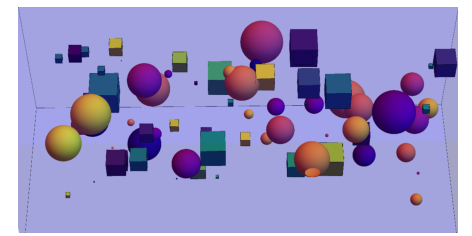
\includegraphics[width=\linewidth]{figures/table1_1.pdf}
    \end{minipage}
    %\end{minipage}
    \\  \hline
    %\begin{minipage}[t]{5cm}
      1. Autonomous Motion
    %\end{minipage}
  
      &
      \begin{minipage}{.15\textwidth}
      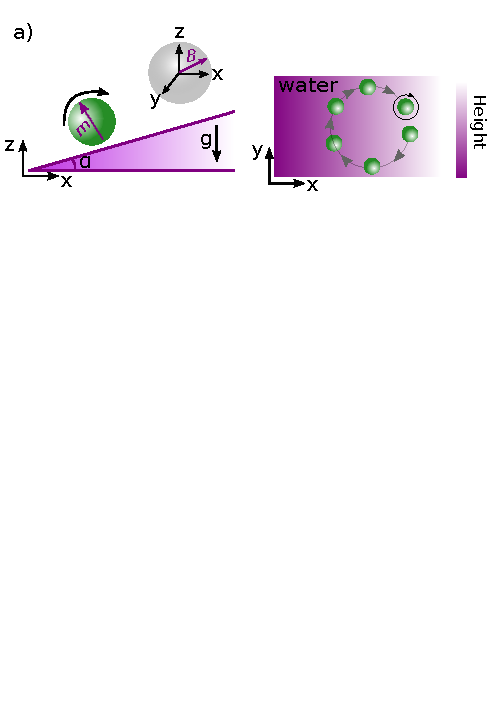
\includegraphics[width=\linewidth]{figures/5_1.pdf}
    \end{minipage}
    %\end{minipage}
    \\  \hline
    %\begin{minipage}[t]{5cm}
      2.Autonomous Coordination
    
      &
      \begin{minipage}{.15\textwidth}
      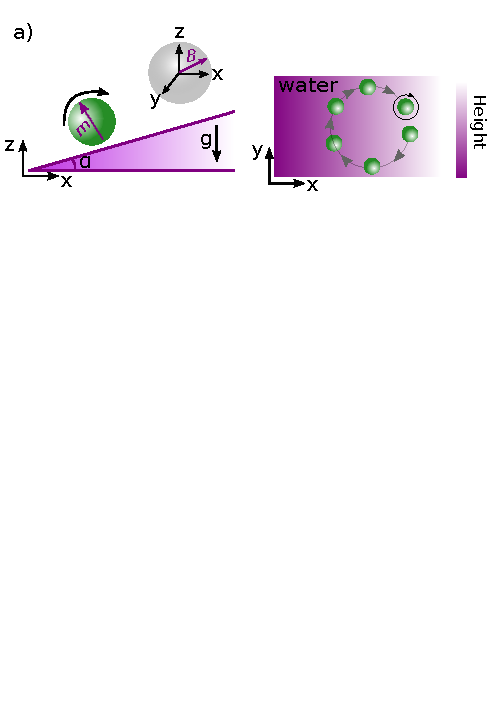
\includegraphics[width=\linewidth]{figures/5_1.pdf}
    \end{minipage}
    %\end{minipage}
    \\  \hline
    %\begin{minipage}[t]{5cm}
      3$^{minus}$. Supervised  Autonomous  Navigation  
    
      &
      \begin{minipage}{.15\textwidth}
      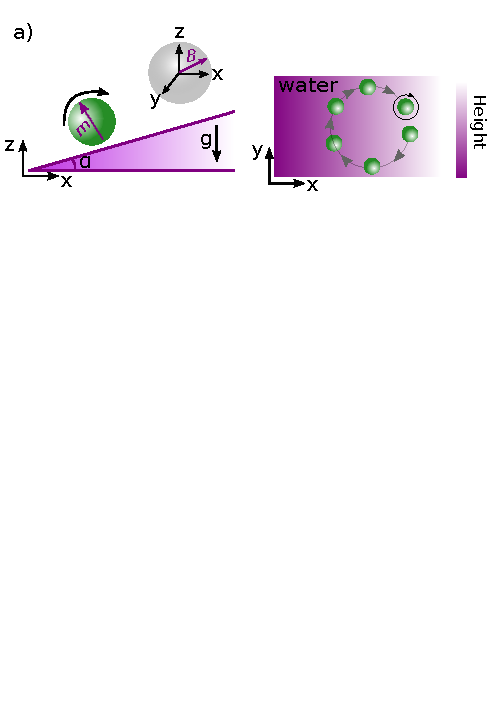
\includegraphics[width=\linewidth]{figures/5_1.pdf}
    \end{minipage}
    %\end{minipage}
    \\  \hline
    %\begin{minipage}[t]{5cm}
      3$^{plus}$. Unsupervised Autonomous Navigation 
   
      
      &
      \begin{minipage}{.15\textwidth}
      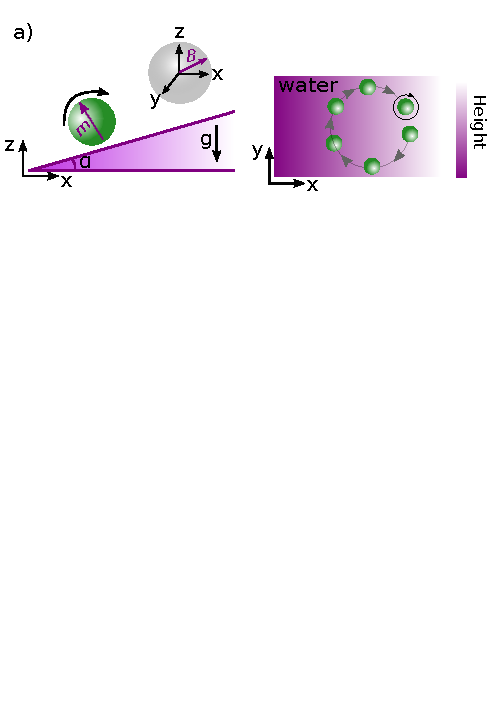
\includegraphics[width=\linewidth]{figures/5_1.pdf}
    \end{minipage}
    %\end{minipage}
    \\ \hline
    %\begin{minipage}[t]{5cm}
      4. Autonomous Communication
    
      &
      \begin{minipage}{.15\textwidth}
      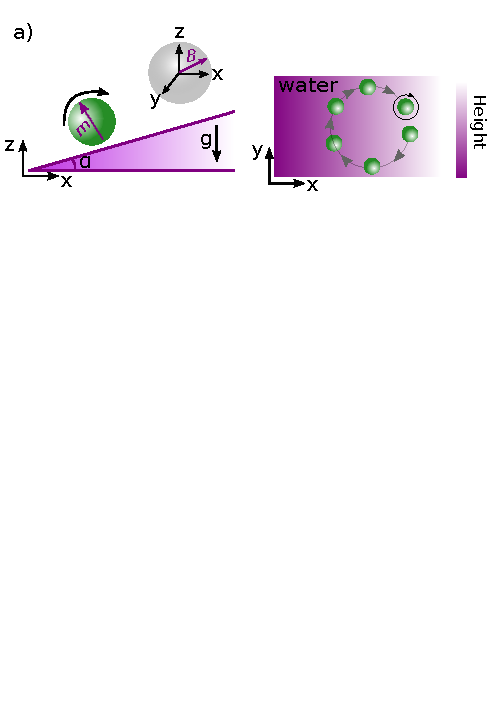
\includegraphics[width=\linewidth]{figures/5_1.pdf}
    \end{minipage}
    %\end{minipage}
    \\ \hline
    %\begin{minipage}[t]{5cm}
      5. Colloid Artificial Intelligent: 
  
      &
      \begin{minipage}{.15\textwidth}
      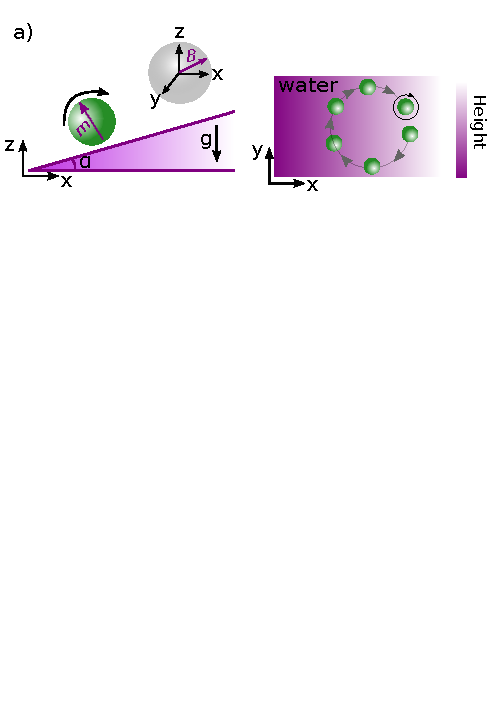
\includegraphics[width=\linewidth]{figures/5_1.pdf}
    \end{minipage}
    %\end{minipage}
    \\ \hline
    
    
    
  \end{tabular}
  \caption{Automation level of colloid robot}\label{tbl:myLboro}
\end{table}



\section{A state of art review on colloid robots }
It is not clear which paper first mentioned  similar idea of colloid scale robotics(the basic concept of  small scale machines can be tracked to Richard Feynman's famous paper,\textit{There's plenty of room at the bottom}\cite{feynman1960there}). The current research wave in the past decade on colloid robot is triggered by the discovery of self propulsion active colloid particle in chemical fuels \cite{paxton2004catalytic}. In 2004, scientist from Penn State University found chemical fuel(they use hydrogen peroxide, $H_2O_2$ in the first paper) can drive  gold-platinum bimetallic nanorods' autonomous motion. The asymmetric different chemical reactions , which happen at different end of nanorod,  lead to a net flow fluid near the surface of nanorod. This pioneer research then attracted lots of attention in different research field beyond chemistry such as soft condensed matter physics\cite{Marchetti2013}, materials science\cite{han2018engineering}, applied math\cite{fodor2016far} and engineering research\cite{sitti2015biomedical}. More than tens of thousands papers related to the autonomous behaviors of colloids have been published since then. However, most of these research papers either experiment or theory only realize the first 2 level automation(autonomous motion and coordination) in colloid robots. Only a few of them realize the supervise/unsupervised autonomous navigation function. From our knowledge, the higher level's automation is still challenging, and should be the main research direction in the future. In the following content, we are going to give a short state-of-art of art review on both experiment approach to colloid robots as well as new theories and simulation methods towards colloid robots. In this short review, I have no intention and interests to rephrase and cover all the research papers on colloid robots like an encyclopedia book. Instead,  I will focus on the main physics, chemistry and engineering ideas behind these papers. 
\subsection{Experiment Approach}
\textbf{Fabrication}  High throughput nano/micro scale fabrication technologies in semiconductor manufacturing industry now can make 3-D structure even smaller than 5$nm$.\cite{mokhlesi2010three} These fancy technologies to make CPU and memory can be transplanted directly to make colloid robots of almost any desired size, shape and component in clean room.\cite{koman2018colloidal} A typical fabrication process mainly including lithography to make patterns as sacrificing models, etching to remove unnecessary materials and deposition to introduce new materials. Multi-layer processing can be designed and optimized to make high dimension and complex structure such as spiral shape\cite{zhang2009artificial}. After the colloid robots are fabricated on the wafer, they can be harvested from the silica surface with etching technology or simply physical removal. For the detailed process of fabrication, I would like to refer readers to these 3 comprehensive reviews\cite{wong2016synthetic,wang2017emerging, zha2018tubular}. Chemists and material scientists also contributed creative chemical synthesis methods to make colloid scale complex structure with one-pot high-throughput\cite{youssef2016shape,gong2017patchy,wang2019active}. One challenge for colloid robot's fabrication is to   make  colloid scale soft(or shape changing) structure with complex component component. liquid crystal, hydrogel gel, droplet and silica polymer with self assembly property are promising candidate materials for micro/nano scale soft structure. \cite{leong2009tetherless,denkov2015self,zhang2017printing,wei2019molecular}. Another fabrication challenge is to make bio-hybrid colloid robots,where experimental biologist can provide invaluable experience and knowledge.\cite{stanton2016biohybrid,magdanz2013development}

\textbf{Actuation} Autonomous motion is the most fundamental characteristic of colloid robots, making colloid robots real machines instead of simple colloid particles. Colloid robots can harness energy from environment and convert energy 


Chemical reaction and external fields are both used to powering the motion of active matters.Asymmetric Chemical Reactions happen on isotropic particles generate chemical's gradient or bubbles to drive the motion of active mater \cite{shklyaev2016harnessing,parmar2018micro}. Besides chemical reactions, electric field, magnetic field and acoustic field are commonly used  to drive active matter, which has less fluctuation trajectories comprared to chemical reaction method \cite{han2018engineering,ren2018two}. active matter system also have a very low efficiency of energy utilization with mass amount of heat dissipation.\cite{wang2013understanding} Some research have shown some active matter can do self-regulate motion by adapting its shape with the environment conduction such as temperature and light intensity.\cite{tu2017self,li2018light} Collective behaviors are usually existed in active matter system like birds' swarm and fish's flock \cite{wang2015one}. The active matters shows emergent patterns such as dynamic clustering and phase separation.\cite{ginot2018aggregation} 

\textbf{Coordination}

\textbf{Navigation}

\subsection{Theory and simulation}
Richard Feynman said "What I cannot create, I do not understand." to emphasise the importance of fundamental understanding of science.This is also true for the  research in colloid robots  
\textbf{physics law of nonequilibrium }

\textbf{hydrodynamics}

\textbf{multi physics field solution }

\textbf{optimization}

%\textbf{Potential Application }